\section{Conics}

Conics are geometric shapes that result from the intersection of cones with planes. 
They include circles, ellipses, parabolas, and hyperbolas, as depicted in the following figure:
\begin{figure}[H]
    \centering
    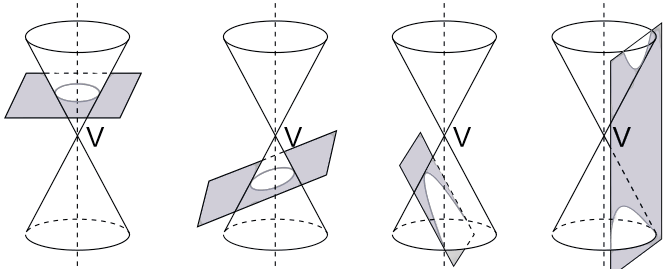
\includegraphics[width=0.5\linewidth]{images/conics.png}
\end{figure}
\begin{definition}
    A point $x$ is considered to be on a \emph{conic} $C$ if it satisfies a homogeneous quadratic equation of the form:
    \[x^TCx=0\]
    Where $C$ is a symmetric matrix is a symmetric matrix, which is a convention.
\end{definition}
Conics are curves described by second-degree equations in the plane. 
In Euclidean coordinates, a conic can be expressed as:
\[aX^2+bXY+cY^2+dX+eY+f=0\]
In homogeneous coordinates, it becomes:
\[ax^2+bxy+cy^2+dxw+eyw+fw^2=0\]
Alternatively, it can be represented in matrix form as:
\[x^T \begin{bmatrix} a & b/2 & d/2 \\ b/2 & c & e/2 \\ d/2 & e/2 & f \end{bmatrix} x=0\]
Conics have five degrees of freedom, which means that five points are required to uniquely define a conic.
\begin{example}
    A circle can be expressed in Cartesian coordinates as:
    \[(X-X_0)^2+(Y-Y_0)^2-r^2=0\]
    In homogeneous coordinates, it is represented as:
    \[  \begin{bmatrix} x & y & w \end{bmatrix}
        \begin{bmatrix} 1 & 0 & -X_0 \\ 0 & 1 & -Y_0 \\ -X_0 & -Y_0 & X_0^2+Y_0^2-r^2 \end{bmatrix}
        \begin{bmatrix} x \\ y \\ w \end{bmatrix} = 0
    \]
\end{example}

When you have a quadratic equation representing a conic and a linear equation for a line, their intersection results in a second-degree equation for the point $x$. 
Consequently, there will always be two intersection points between a line and a conic. 
These intersection points can fall into one of the following categories:
\begin{itemize}
    \item Real and distinct: this occurs when the line and conic intersect at two separate, real points.
    \item Real and coincident: in this case, the line and conic intersect at a single real point, but it is a repeated or double root of the equation.
    \item Complex and distinct: the intersection points are two complex conjugate points.
    \item Complex and coincident: the line and conic intersect at a single complex point, and it is a repeated or double root.
\end{itemize}
This behavior is due to the fundamental theorem of algebra, which guarantees that a second-degree equation will have exactly two solutions when considering complex numbers.
\begin{figure}[H]
    \centering
    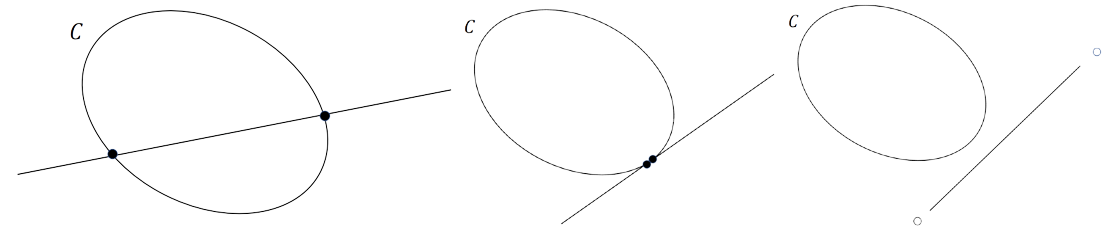
\includegraphics[width=0.75\linewidth]{images/intersection.png}
    \caption{Intersection with two real roots, two coincident roots and two imaginary roots}
\end{figure}
The intersection between the line at infinity and a conic results in the following scenarios:
\begin{itemize}
    \item Parabola: when there are two coincident solutions, indicating the point at infinity along the axis.
    \item Ellipse: when there are two complex-conjugate solutions, meaning there are no real solutions.
    \item Hyperbola: when there are two real and distinct solutions, representing lines that serve as the asymptotes.
\end{itemize}

\subsection*{Circular points}
\begin{example}
    When we intersect a circumference and the line at infinity, we obtain the following system:
    \[\begin{cases}
        x^2-2X_0w+X_0^2w^2+y^2-2Y_0w+Y_0^2w^2-r^2w^2=0 \\
        w=0
    \end{cases}\]
    This system simplifies to: 
    \[x^2+y^2=0\]
    It's evident that the parameters of the circumference (center and radius) have disappeared from the equation. 
    Consequently, the two intersection points are the same for all circumferences.    
\end{example}
\newpage
\begin{definition}
    The two intersection points remain the same for all circumferences when intersected with the line at infinity are referred to as the \emph{circular points}.
    These points are defined as:
    \[I=\begin{bmatrix} 1 \\ i \\ 0 \end{bmatrix} \:\:\:\:\:\: J=\begin{bmatrix} 1 \\ -i \\ 0 \end{bmatrix}\]
\end{definition}

\subsection*{Polar line}
\begin{definition}
    Given a point $y$ and a conic $C$ in the plane, the line $l=Cy$ is called the \emph{polar line} of point $y$ with respect to the conic $C$. 
\end{definition}
\begin{figure}[H]
    \centering
    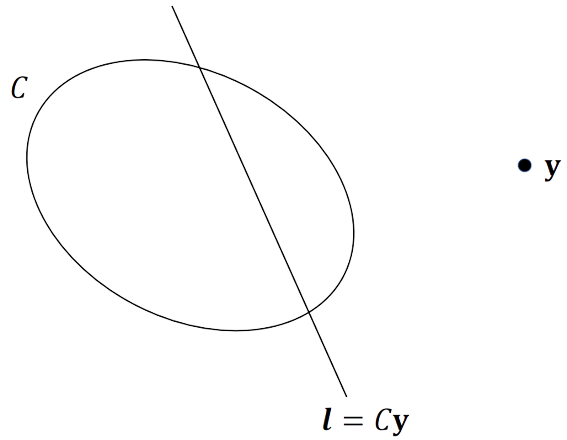
\includegraphics[width=0.3\linewidth]{images/polar.png}
    \caption{Example of polar line}
\end{figure}

\subsection*{Harmonic tuples}
\begin{definition}
    A 4-tuple of co-linear points A, B, C, D, whose cross ratio is = -1, is referred to as a \emph{harmonic tuple}. 
\end{definition}
This specific value of the cross ratio is also shared by other 4-tuples of co-linear points. 
A notable example is:
\[\left( T,Z,\textnormal{mid\_point}(Y,Z),P(\textnormal{at the infinity}) \right)\]
Furthermore, if $(A, B, C, D)$ is a harmonic 4-tuple, then $(C, D, A, B)$ is also harmonic. 
\begin{definition}
    In a harmonic tuple $(A, B, C, D)$, points $A$ and $B$ are said to be \emph{conjugate} of each other concerning points $C$ and $D$.
\end{definition}
Since the cross ratio of a harmonic tuple is negative, it follows that two conjugate points, $A$ and $B$, concerning $C$ and $D$, are positioned in such a way that one is located within the segment ($C, D$), while the other is situated outside this segment.

\subsection*{Polar line and harmonic tuples}
Take any point $z$ on the polar line $l=Cy$ and then consider the line passing through points $y$ and $z$. 
Let's denote by $x_1$ and $x_2$ the points at which this line intersects the conic.    
\begin{figure}[H]
    \centering
    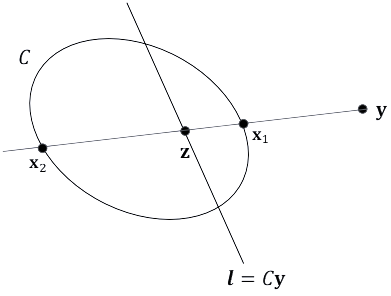
\includegraphics[width=0.25\linewidth]{images/polarharmonic.png}
\end{figure}
\begin{theorem}
    Let $x_1$ and $x_2$ represent the points at which the line passing through $y$ and $z$ intersects the conic $C$. 
    In this case, $y$ and $z$ are conjugate with respect to $x_1$ and $x_2$.     
\end{theorem}
The polar line $l=Cy$ represents the set of points that are conjugate to $y$ with respect to the conic $C$.
More precisely, it includes points that are conjugate with respect to the intersection points of $C$ with any line passing through $y$.

\subsection*{Polar line and tangency points}
As the line through $y$ approaches tangency with the conic $C$, the points $x_1$ and $x_2$ coincide with the points of tangency to $C$. 
Consequently, the conjugate point $z$, which remains within the interval ($x_1,x_2$), also coincides with the tangency point. 
This applies to any line that is tangent to $C$ from the point $y$.
Therefore, we have established that the polar line $l=Cy$ passes through the points of tangency from $y$ to the conic $C$. 

This leads us to the conclusion that if a point $z$ lies on the conic $C$, then point $y$ is one of its conjugates with respect to the same conic. 
The tangent line $lz$ to the conic $C$ passing through point $z$ is the set of points that are conjugate to $z$. 
Therefore, we can assert that $lz$ is the polar line of $z$ with respect to conic $C$.
\begin{figure}[H]
    \centering
    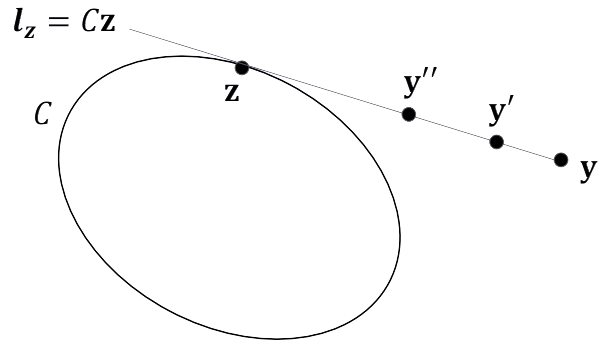
\includegraphics[width=0.4\linewidth]{images/tangentpolar.png}
\end{figure}
In the accompanying illustration, you can observe that the polar line $lz = Cz$ for a point $z$ situated on the conic $C$ corresponds to the tangent line to the conic $C$ at the point $z$.
\begin{example}
    Consider a circumference with radius $r$ centered in the origin of the plane and the point $y={\begin{bmatrix} X & 0 & 1 \end{bmatrix}}^T$. 
    The equation of the polar line is given by:
    \[
    l=Cy=
    \begin{bmatrix}
        1 & 0 & 0 \\
        0 & 1 & 0 \\
        0 & 0 & -r^2
    \end{bmatrix}    
    \begin{bmatrix}
        X \\
        0 \\
        1 
    \end{bmatrix}    
    = 
    \begin{bmatrix}
        X \\
        0 \\
        -r^2 
    \end{bmatrix}  
    \]
    Therefore, the Cartesian equation of the polar line becomes: 
    \[X x-r^2 = 0 \rightarrow x=\dfrac{r^2}{X}\]
    This equation describes a vertical line.
\end{example}

From the previous example, we can conclude that the polar of a point $P$ with respect to a circle is a line that is perpendicular to the line segment connecting the center of the circle to point $P$. 
\begin{example}
    Consider a circumference with radius $r$ centered in the origin of the plane and the point $y={\begin{bmatrix} x & 0 & 0 \end{bmatrix}}^T$.
    The equation of the polar line is given by:
    \[
    l=Cy=
    \begin{bmatrix}
        1 & 0 & 0 \\
        0 & 1 & 0 \\
        0 & 0 & -r^2
    \end{bmatrix}    
    \begin{bmatrix}
        x \\
        0 \\
        0 
    \end{bmatrix}    
    = 
    \begin{bmatrix}
        X \\
        0 \\
        0 
    \end{bmatrix}  
    \]
    Therefore, the Cartesian equation of the polar line becomes: 
    \[X x=0 \rightarrow X=0\]
    This equation describes the diameter of the circumference perpendicular at the direction of the point $y$. 
\end{example}
Tangent lines emerging from a point at infinity are always parallel. 
Consequently, the points of tangency lie along a diameter that is perpendicular to the direction of these parallel tangents.    
\begin{figure}[H]
    \centering
    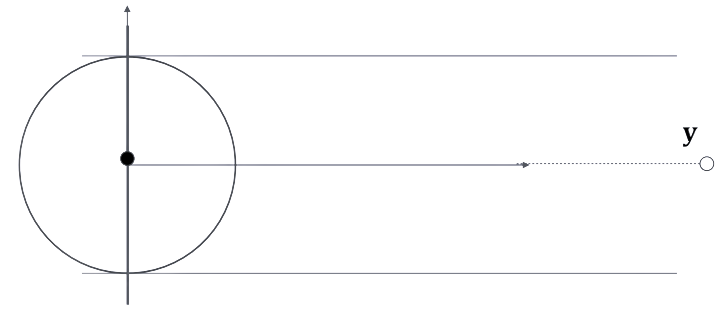
\includegraphics[width=0.5\linewidth]{images/parallel.png}
\end{figure}
\begin{example}
    Consider a circumference with radius $r$ centered in the origin of the plane and the point $y={\begin{bmatrix} x & 0 & 0 \end{bmatrix}}^T$.
    The equation of the polar line is given by:
    \[
    l=Cy=
    \begin{bmatrix}
        1 & 0 & 0 \\
        0 & 1 & 0 \\
        0 & 0 & -r^2
    \end{bmatrix}    
    \begin{bmatrix}
        0 \\
        0 \\
        1 
    \end{bmatrix}    
    = 
    \begin{bmatrix}
        0 \\
        0 \\
        -r^2 
    \end{bmatrix}  
    \]
    Therefore, the Cartesian equation of the polar line becomes: 
    \[-r^2w=0 \rightarrow X=0\]
    This equation describes the line at the infinity. 
\end{example}
Here are the general properties of the polar lines.
\begin{property}
    The polar line of any point at infinity is a diameter.
\end{property}
\begin{property}
    Any diameter goes through the center of the circle.
\end{property}
\begin{property}
    The center is conjugate to every point at infinity.
\end{property}
\begin{property}
    All points at infinity are conjugate to the center.
\end{property}
\begin{property}
    The polar of the center is the line that includes all the points at infinity.
\end{property}
\begin{property}
    The polar line of the center is the line at infinity.
\end{property}

\subsection*{Degenerate conics}
\begin{definition}
    A \emph{non-degenerate conic} is a conic where the matrix $C$ is non-singular, indicating that: 
    \[\textnormal{rank}(C)=3\]

    Conversely, a \emph{degenerate conic} is a conic  for which the matrix $C$ is singular, characterized by: 
    \[\textnormal{rank}(C) < 3\]
\end{definition}
There are two distinct scenarios to consider:
\begin{itemize}
    \item When $\textnormal{rank}(C) = 2$, any symmetric $3 \times 3$ matrix $C$ can be expressed as:
        \[C=lm^T+ml^T\]
        Here, $l$ and $m$ are column vectors. 
        The conic corresponds to the set of points $x$  that satisfy $x^TCx=0$.
        This equation is met when either $x^Tl=0$ or $m^Tx=0$. 
        Consequently, $x$ lies on the union of lines represented by $l$ and $m$
        \begin{figure}[H]
            \centering
            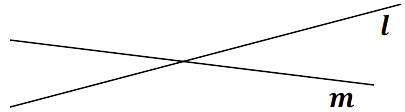
\includegraphics[width=0.25\linewidth]{images/inters.png}
        \end{figure}
    \item When $\textnormal{rank}(C) = 1$, a symmetric $3 \times 3$ matrix $C$ can be expressed as:
        \[C=ll^T\]
        In this case, $l$ is a column vector. 
        The conic consists of the points $x$ that satisfy $x^TCx=0$.
        This equation holds  when $x^Tl=0$ is met (twice). 
        Thus, $x$ is on the repeated line represented by $l$.
        \begin{figure}[H]
            \centering
            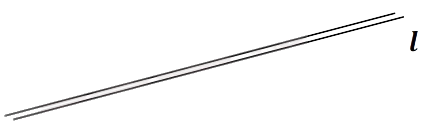
\includegraphics[width=0.25\linewidth]{images/rep.png}
        \end{figure}
\end{itemize}